\chapter{Monte Carlo Simulation}\label{cap:montecarlo}

The modern version of the Monte Carlo method dates back to the
introduction of the first computers and their application during the
years 1940-45 with the purpose of computing neutron diffusion in atomic
bombs.

The Monte Carlo approach was primarily promoted and advanced by physics
researchers Stanislaw Ulam, Nicholas Metropolis and John von Neumann.
They were well aware of the potential of such techniques but it was only
with the first electronic computer - the ENIAC - which was able to solve
differential equations at a tremendous, so far unconceivable speed, the
Monte Carlo method was eventually triggered.

The name Monte Carlo refers to a famous casino in Monaco where Ulam's
uncle used to indulge his gambling passion. The characteristics of
randomness and the repetitive nature of many processes correspond with
the games played in a casino. Note that the famous roulette wheel is
one of the simplest mechanical devices to generate random variables.

Simulation tools find their application mostly in cases where the
inherent complexity of a problem makes the use of other techniques
impossible or where no analytically tractable solution with a
deterministic algorithm is existing. In short, the Monte Carlo method is
a numerical approach which aims for solving mathematical problems by the
simulation of random variables.

Monte Carlo simulations are widely used in many fields: Engineering,
Physics, Computational biology, Computer graphics, Applied statistics and 
Artificial intelligence for games.

It started to be en vogue in financial mathematics in the 1980s,
particularly when the theories of the random walk of asset prices came
up.

%The modern version of the Monte Carlo method was invented in the late
%1940s by Stanislaw Ulam, while he was working on nuclear weapon
%projects at the Los Alamos National Laboratory.

%Monte Carlo methods, or experiments, are a broad class of computational
%algorithms that rely on repeated random sampling to obtain numerical
%results; the underlying concept is to use randomness to solve problems
%that might be deterministic in principle. Monte Carlo methods are mainly
%used in three problem classes: optimization, numerical integration, and
%generating draws from a probability distribution.

In this Chapter we will review it and see some useful application.

\section{The Algorithm}\label{whats-monte-carlo-simulation}

Monte Carlo (MC) methods are used when a closed-form solution for a
property being studied cannot be developed.

A MC simulation performs analysis by building a model and producing 
results by substituting a random variable with its PDF
for any factor that has inherent uncertainty. 
It then calculates results over and over, each time using a different set of
random values from the forementioned probability distributions. 
Depending upon the number of uncertainties and the ranges specified for them,
a Monte Carlo simulation could involve thousands or tens of thousands of
calculations before it is complete. Finally the simulation
produces distributions of possible outcome values.

A MC method/algorithm then can be described as follows: 
\begin{itemize}
	\item  select a domain \(\Omega\) for the inputs (probability distributions for our
	factors); 
	\item generate random inputs from this domain \(\Omega\);
	\item perform
	a deterministic computation with those inputs;
	\item aggregate the results.
\end{itemize}

In the next Sections we will see each point applied to practical examples.

\section{Pseudo-Random Numbers}\label{pseudo-random-numbers}

The second point above implies that Monte Carlo methods require 
large amounts of random numbers to
generate the inputs, and it was their use that spurred the development
of pseudo-random number generators. 

Every programming language has libraries that
allows to produce huge series of random numbers (with a periodicity of
\(2^{19937}\)). These series are calculated by algorithms that take as
input a \emph{seed} which determines them uniquely. This means
that choosing the same seed you will produce the same set of numbers
every time (which is great for debugging purposes).

In \texttt{python} one of the available modules to generate random numbers is \texttt{random} which has, among others, the following useful functions:
\begin{itemize}
\tightlist
\item
  \texttt{seed} set the seed of the random number generator;
\item
  \texttt{random} returns a random number between 0 and 1 (with uniform
  probability);
\item
  \texttt{randint(min,\ max)} returns an integer random number between
  \texttt{min} and \texttt{max} (with uniform probability);
\item
  \texttt{sample(aList,\ k=n)} samples n elements from the list
  \texttt{aList}.
\end{itemize}
As usual for a more detailed description check \texttt{help(random)}.
The following example shows an application of these functions besides the effect of  changing the seed of the random number generator.

\begin{tcolorbox}[breakable, size=fbox, boxrule=1pt, pad at break*=1mm,colback=cellbackground, colframe=cellborder]
\begin{Verbatim}[commandchars=\\\{\}]
\PY{k+kn}{import} \PY{n+nn}{random} 

\PY{n}{random}\PY{o}{.}\PY{n}{seed}\PY{p}{(}\PY{l+m+mi}{1}\PY{p}{)}
\PY{n+nb}{print} \PY{p}{(}\PY{l+s+s2}{\PYZdq{}}\PY{l+s+s2}{seed is 1}\PY{l+s+s2}{\PYZdq{}}\PY{p}{)}
\PY{n+nb}{print}\PY{p}{(}\PY{n}{random}\PY{o}{.}\PY{n}{random}\PY{p}{(}\PY{p}{)}\PY{p}{)}
\PY{n+nb}{print}\PY{p}{(}\PY{n}{random}\PY{o}{.}\PY{n}{random}\PY{p}{(}\PY{p}{)}\PY{p}{)}

\PY{n}{random}\PY{o}{.}\PY{n}{seed}\PY{p}{(}\PY{l+m+mi}{2}\PY{p}{)}
\PY{n+nb}{print} \PY{p}{(}\PY{l+s+s2}{\PYZdq{}}\PY{l+s+s2}{seed is 2}\PY{l+s+s2}{\PYZdq{}}\PY{p}{)}
\PY{n+nb}{print}\PY{p}{(}\PY{n}{random}\PY{o}{.}\PY{n}{random}\PY{p}{(}\PY{p}{)}\PY{p}{)}
\PY{n+nb}{print}\PY{p}{(}\PY{n}{random}\PY{o}{.}\PY{n}{random}\PY{p}{(}\PY{p}{)}\PY{p}{)}

\PY{n}{random}\PY{o}{.}\PY{n}{seed}\PY{p}{(}\PY{l+m+mi}{1}\PY{p}{)}
\PY{n+nb}{print} \PY{p}{(}\PY{l+s+s2}{\PYZdq{}}\PY{l+s+s2}{seed is 1 again}\PY{l+s+s2}{\PYZdq{}}\PY{p}{)}
\PY{n+nb}{print}\PY{p}{(}\PY{n}{random}\PY{o}{.}\PY{n}{random}\PY{p}{(}\PY{p}{)}\PY{p}{)}
\PY{n+nb}{print}\PY{p}{(}\PY{n}{random}\PY{o}{.}\PY{n}{random}\PY{p}{(}\PY{p}{)}\PY{p}{)}

\PY{n+nb}{print}\PY{p}{(}\PY{n}{random}\PY{o}{.}\PY{n}{randint}\PY{p}{(}\PY{l+m+mi}{1}\PY{p}{,} \PY{l+m+mi}{10}\PY{p}{)}\PY{p}{)}
\PY{n}{aList} \PY{o}{=} \PY{p}{[}\PY{l+s+s1}{\PYZsq{}}\PY{l+s+s1}{a}\PY{l+s+s1}{\PYZsq{}}\PY{p}{,} \PY{l+s+s1}{\PYZsq{}}\PY{l+s+s1}{b}\PY{l+s+s1}{\PYZsq{}}\PY{p}{,} \PY{l+s+s1}{\PYZsq{}}\PY{l+s+s1}{c}\PY{l+s+s1}{\PYZsq{}}\PY{p}{,} \PY{l+s+s1}{\PYZsq{}}\PY{l+s+s1}{d}\PY{l+s+s1}{\PYZsq{}}\PY{p}{,} \PY{l+s+s1}{\PYZsq{}}\PY{l+s+s1}{f}\PY{l+s+s1}{\PYZsq{}}\PY{p}{]}
\PY{n+nb}{print} \PY{p}{(}\PY{n}{random}\PY{o}{.}\PY{n}{sample}\PY{p}{(}\PY{n}{aList}\PY{p}{,} \PY{n}{k}\PY{o}{=}\PY{l+m+mi}{2}\PY{p}{)}\PY{p}{)}

seed is 1
0.13436424411240122
0.8474337369372327
seed is 2
0.9560342718892494
0.9478274870593494
seed is 1 again
0.13436424411240122
0.8474337369372327
2
['c', 'a']
    \end{Verbatim}
\end{tcolorbox}

The next lines of code show instead how to draw a uniform distribution. Figure~\ref{fig:uniform_dist} shows the result.

 \begin{tcolorbox}[breakable, size=fbox, boxrule=1pt, pad at break*=1mm,colback=cellbackground, colframe=cellborder]
\begin{Verbatim}[commandchars=\\\{\}]
\PY{n}{numbers} \PY{o}{=} \PY{p}{[}\PY{p}{]}
\PY{k}{for} \PY{n}{\PYZus{}} \PY{o+ow}{in} \PY{n+nb}{range}\PY{p}{(}\PY{l+m+mi}{10000}\PY{p}{)}\PY{p}{:}
  \PY{n}{numbers}\PY{o}{.}\PY{n}{append}\PY{p}{(}\PY{n}{random}\PY{o}{.}\PY{n}{randint}\PY{p}{(}\PY{l+m+mi}{0}\PY{p}{,} \PY{l+m+mi}{5}\PY{p}{)}\PY{p}{)}

\PY{k+kn}{from} \PY{n+nn}{matplotlib} \PY{k}{import} \PY{n}{pyplot} \PY{k}{as} \PY{n}{plt}
\PY{n}{plt}\PY{o}{.}\PY{n}{hist}\PY{p}{(}\PY{n}{numbers}\PY{p}{,} \PY{l+m+mi}{6}\PY{p}{,} \PY{n+nb}{range}\PY{o}{=}\PY{p}{[}\PY{o}{\PYZhy{}}\PY{l+m+mf}{0.5}\PY{p}{,} \PY{l+m+mf}{5.5}\PY{p}{]}\PY{p}{)}
\PY{n}{plt}\PY{o}{.}\PY{n}{title}\PY{p}{(}\PY{l+s+s2}{\PYZdq{}}\PY{l+s+s2}{Uniform distribution from randint}\PY{l+s+s2}{\PYZdq{}}\PY{p}{)}
\PY{n}{plt}\PY{o}{.}\PY{n}{show}\PY{p}{(}\PY{p}{)}
\end{Verbatim}
\end{tcolorbox}

\begin{figure}[h]
\centering
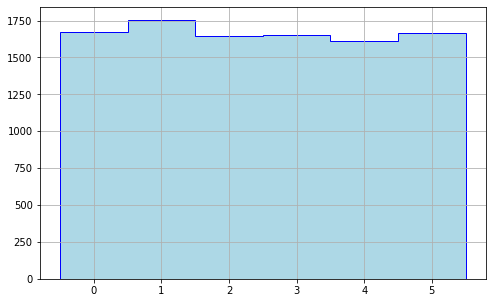
\includegraphics[width=0.7\textwidth]{figures/lesson4_3_0.png}
\caption{Uniform distribution generated with \texttt{random.randint} function.}
\label{fig:uniform_dist}
\end{figure}
    
Another useful module that we will use later to generate random numbers is \texttt{numpy}. It has similar functionalities to \texttt{random} but in some cases it fits better to our needs.    
Below an example with \texttt{numpy.random.normal} which allows to throw random numbers according to a normal distribution
(\(\mathcal{N}(0, 1)\)), its plot is shown in Fig.~\ref{fig:gauss_dist}.

\begin{tcolorbox}[breakable, size=fbox, boxrule=1pt, pad at break*=1mm,colback=cellbackground, colframe=cellborder]
\begin{Verbatim}[commandchars=\\\{\}]
\PY{k+kn}{from} \PY{n+nn}{numpy}\PY{n+nn}{.}\PY{n+nn}{random} \PY{k}{import} \PY{n}{normal}
\PY{k+kn}{from} \PY{n+nn}{matplotlib} \PY{k}{import} \PY{n}{pyplot} \PY{k}{as} \PY{n}{plt}

\PY{n}{gauss} \PY{o}{=} \PY{p}{[}\PY{p}{]}
\PY{k}{for} \PY{n}{\PYZus{}} \PY{o+ow}{in} \PY{n+nb}{range}\PY{p}{(}\PY{l+m+mi}{50000}\PY{p}{)}\PY{p}{:}
  \PY{n}{gauss}\PY{o}{.}\PY{n}{append}\PY{p}{(}\PY{n}{normal}\PY{p}{(}\PY{p}{)}\PY{p}{)}
  
\PY{n}{plt}\PY{o}{.}\PY{n}{hist}\PY{p}{(}\PY{n}{gauss}\PY{p}{,} \PY{l+m+mi}{100}\PY{p}{,} \PY{n+nb}{range}\PY{o}{=}\PY{p}{[}\PY{o}{\PYZhy{}}\PY{l+m+mi}{4}\PY{p}{,} \PY{l+m+mi}{4}\PY{p}{]}\PY{p}{)}
\PY{n}{plt}\PY{o}{.}\PY{n}{title}\PY{p}{(}\PY{l+s+s2}{\PYZdq{}}\PY{l+s+s2}{Example of Gaussian distribution from numpy}\PY{l+s+s2}{\PYZdq{}}\PY{p}{)}
\PY{n}{plt}\PY{o}{.}\PY{n}{show}\PY{p}{(}\PY{p}{)}
\end{Verbatim}
\end{tcolorbox}

 \begin{figure}
   \centering
   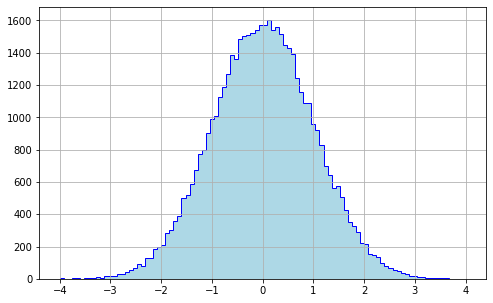
\includegraphics[width=0.7\textwidth]{figures/lesson4_5_0.png}
   \caption{Normal distribution generated with \texttt{numpy.random.normal} function.}
\label{fig:gauss_dist}
 \end{figure}

%\hypertarget{acceptance-rejection-method}{%
%\subsubsection{Acceptance-Rejection
%	Method}\label{acceptance-rejection-method}}
%
%The acceptance-rejection method was proposed by von Neumann in 1951 and
%is used in order to generate random variables that follow a probability
%density function denoted by \(f(x)\). Since we are occasionally
%struggling in inverting the CDF that corresponds to our \(f(x)\), the
%just discussed inverse transform method loses ground and the
%acceptance-rejection method is applied.
%
%Given a so called target distribution \(f(x)\), the acceptance-rejection
%method generates samples according to \(f(x)\) by first of all
%generating samples from a more suitable distribution \(g(y)\).
%Afterwards a random subset of these generated samples is rejected
%according to certain rejection rules. Thereby the choice of this
%rejection rule, or let us call it rejection approach, will be decisive
%if the accepted samples will eventually be distributed according to
%\(f(x)\). The property \(f(x) \leq c\cdot g(x)\), for some constant
%\(c\), tells us now how to generate samples from \(g(y)\). Therefore, we
%conclude that in the acceptance-rejection method a sample \(Y\) is
%generated from \(g\) and at the same time accepted with probability
%\(f(Y)/cg(Y)\). The generic implementation, i.e.~the algorithm of the
%acceptance-rejection method that we can use to sample from density \(f\)
%using candidates from \(g\), can be stated as follows:
%
%\begin{enumerate}
%\def\labelenumi{\arabic{enumi}.}
%\tightlist
%\item
%generate the sample \(Y\) from the distribution with density \(g\)
%\item
%generate \(u\) from \(U[0,1]\), which must be independent of \(Y\)
%\item
%if \(u\leq f(Y)/cg(Y)\), then deliver \(X = Y\), otherwise return to
%step 1.
%\end{enumerate}

\section{Practical Examples of Monte Carlo
Simulation}\label{example-of-monte-carlo-simulation}

In this Section we go through some applications of the Monte Carlo method.

\subsection{Probability to draw two kings from a deck}
Using a frequentist approach, we can calculate the
probability of an event as the ratio of the number of favorable outcomes
of an experiment (number of successes) and the number of all possible
outcomes. 

Imagine we would like to determine the probability of drawing two kings from a standard deck of cards.
At the beginning we have 40 cards (i.e. the entire deck) with 4 possible kings so the probability to get a king is $4/40$. Next, assuming we got a king the first time, we are left with 39 cards and 3 kings only so the probability to get the second king is $3/39$. Since we want both events to happen, the final probability is the product of the two contributions:

\[P_\textrm{two kings} = \frac{4}{40} \cdot \frac{3}{39} = \frac{1}{130} \approx 0.0077\]

Let's now try with a MC simulation following the steps outlined above and check if we get the same number.
\begin{itemize}
\item \emph{Define a domain of possible inputs}: in this case the domain is a deck of cards. With the \texttt{*} operator a list can be easily repeated many times. In this case it is enough four times, once for each suit (in the example we also set the seed to 1 to make it reproducible).

\begin{tcolorbox}[breakable, size=fbox, boxrule=1pt, pad at break*=1mm,colback=cellbackground, colframe=cellborder]
\begin{Verbatim}[commandchars=\\\{\}]
\PY{k+kn}{from} \PY{n+nn}{random} \PY{k}{import} \PY{n}{sample}\PY{p}{,} \PY{n}{choices}\PY{p}{,} \PY{n}{seed}

\PY{n}{seed}\PY{p}{(}\PY{l+m+mi}{1}\PY{p}{)}
\PY{n}{deck} \PY{o}{=} \PY{p}{[}\PY{l+s+s2}{\PYZdq{}}\PY{l+s+s2}{A}\PY{l+s+s2}{\PYZdq{}}\PY{p}{,} \PY{l+s+s2}{\PYZdq{}}\PY{l+s+s2}{2}\PY{l+s+s2}{\PYZdq{}}\PY{p}{,} \PY{l+s+s2}{\PYZdq{}}\PY{l+s+s2}{3}\PY{l+s+s2}{\PYZdq{}}\PY{p}{,} \PY{l+s+s2}{\PYZdq{}}\PY{l+s+s2}{4}\PY{l+s+s2}{\PYZdq{}}\PY{p}{,} \PY{l+s+s2}{\PYZdq{}}\PY{l+s+s2}{5}\PY{l+s+s2}{\PYZdq{}}\PY{p}{,} \PY{l+s+s2}{\PYZdq{}}\PY{l+s+s2}{6}\PY{l+s+s2}{\PYZdq{}}\PY{p}{,} \PY{l+s+s2}{\PYZdq{}}\PY{l+s+s2}{7}\PY{l+s+s2}{\PYZdq{}}\PY{p}{,} \PY{l+s+s2}{\PYZdq{}}\PY{l+s+s2}{J}\PY{l+s+s2}{\PYZdq{}}\PY{p}{,} \PY{l+s+s2}{\PYZdq{}}\PY{l+s+s2}{Q}\PY{l+s+s2}{\PYZdq{}}\PY{p}{,} \PY{l+s+s2}{\PYZdq{}}\PY{l+s+s2}{K}\PY{l+s+s2}{\PYZdq{}}\PY{p}{]} \PY{o}{*} \PY{l+m+mi}{4}
 \end{Verbatim}
\end{tcolorbox}

\item \emph{Generate inputs randomly from a probability distribution over the defined domain}: which means we draw randomly cards with uniform probability since the deck is fair and all cards have the same probability to be drawn. 
We plan to do 1 million simulations, each time with the \texttt{sample} function we pick up two cards with uniform probability from our virtual deck (for debugging purpose the first 10 trials are printed).

\begin{tcolorbox}[breakable, size=fbox, boxrule=1pt, pad at break*=1mm,colback=cellbackground, colframe=cellborder]
\begin{Verbatim}[commandchars=\\\{\}]
\PY{n}{trials} \PY{o}{=} \PY{l+m+mi}{1000000}
\PY{n}{successes} \PY{o}{=} \PY{l+m+mi}{0}

\PY{k}{for} \PY{n}{i} \PY{o+ow}{in} \PY{n+nb}{range}\PY{p}{(}\PY{n}{trials}\PY{p}{)}\PY{p}{:}
  \PY{n}{cards} \PY{o}{=} \PY{n}{sample}\PY{p}{(}\PY{n}{deck}\PY{p}{,} \PY{n}{k}\PY{o}{=}\PY{l+m+mi}{2}\PY{p}{)}
  \PY{k}{if} \PY{n}{i} \PY{o}{\PYZlt{}} \PY{l+m+mi}{10}\PY{p}{:}
    \PY{n+nb}{print} \PY{p}{(}\PY{n}{cards}\PY{p}{)}
\end{Verbatim}
\end{tcolorbox}

\item \emph{Perform a deterministic computation on the generated inputs}: this step is particularly simple in this case, we just need to check if the draw is \texttt{['K', 'K']} and in case increase the counter of successes.

\begin{tcolorbox}[breakable, size=fbox, boxrule=1pt, pad at break*=1mm,colback=cellbackground, colframe=cellborder]
\begin{Verbatim}[commandchars=\\\{\}]
  \PY{k}{if} \PY{n}{cards} \PY{o}{==} \PY{p}{[}\PY{l+s+s2}{\PYZdq{}}\PY{l+s+s2}{K}\PY{l+s+s2}{\PYZdq{}}\PY{p}{,} \PY{l+s+s2}{\PYZdq{}}\PY{l+s+s2}{K}\PY{l+s+s2}{\PYZdq{}}\PY{p}{]}\PY{p}{:}
    \PY{n}{successes} \PY{o}{+}\PY{o}{=} \PY{l+m+mi}{1}
 \end{Verbatim}
\end{tcolorbox}

\item \emph{Aggregate the results}: finally we just print successes/trials which is the sought probability.

\begin{tcolorbox}[breakable, size=fbox, boxrule=1pt, pad at break*=1mm,colback=cellbackground, colframe=cellborder]
\begin{Verbatim}[commandchars=\\\{\}]
\PY{n+nb}{print} \PY{p}{(}\PY{l+s+s2}{\PYZdq{}}\PY{l+s+s2}{The probability to draw two kings is }\PY{l+s+si}{\PYZob{}:.4f\PYZcb{}}\PY{l+s+s2}{\PYZdq{}}\PY{o}{.}\PY{n}{format}\PY{p}{(}\PY{n}{successes}\PY{o}{/}\PY{n}{trials}\PY{p}{)}\PY{p}{)}

['Q', '7']
['5', '7']
['J', '2']
['Q', 'A']
['5', '4']
['7', '2']
['2', '5']
['J', 'Q']
['A', 'Q']
['J', '5']
The probability to draw two kings is 0.0077
    \end{Verbatim}
\end{tcolorbox}
\end{itemize}
The result is in agreement with our theoretical expectations.

Since we relied on a frequentist approach naively we can say that the
lower is the probability we need to estimate the higher has to be the
number of simulated trials. This is because to get a reasonable number
of "success" so that the uncertainty in the probability is small, we
have to try many times. This is apparent playing with the number of
trials in the above simulation. 

This is also the main reason why, despite its undoubted power, Monte Carlo simulation is not always the best approach to follow.
Many times indeed the simulation of an experiment requires a lot of computing resources (and time) and it may not be practical to embark into such a large simulation.

\subsection{Determine \(\pi\)}\label{determine-pi}

Also in this case we know what to expect:
\(\pi\approx 3.141592653589793\ldots\) In order to get an estimate through MC
simulation a straightforward geometric approach has to be considered. Imagine a circle of diameter \(D\) which is inscribed in a square with side length \(D\), see Fig.~\ref{fig:circle_inscribed}.

\begin{figure}[htb]
	\centering
	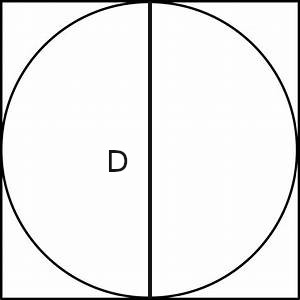
\includegraphics[width=0.3\textwidth]{figures/circle_inscribed.jpeg}
	\caption{A circle of diameter $D$ inscribed in a square.}
	\label{fig:circle_inscribed}
\end{figure}

Computing the ratio of the area of the 2 figures

\begin{equation}
\frac{\textrm{Area Circle}}{\textrm{Area Square}} = \frac{\pi D^2/4}{D^2} = \frac{\pi}{4} 
\end{equation}

The algorithm to approximate \(\pi\) should be

\begin{itemize}
	\item select 2 random numbers, \(x_1\) and \(x_2\), from the interval
\([0,D]\); 
\item determine if the point defined by the ordered pair
\((x_1, x_2)\) lies within or on the circle, keeping track of the total number of
tested points and of those satisfying the condition \(D \le\sqrt{x_1^2 + x_2^2}\); 
\item approximate the ratio of the areas by the number of points within or on
the circle divided by the total number of tested points; 
\item multiply the approximated area by 4 to get \(\pi\).
\end{itemize}

\begin{tcolorbox}[breakable, size=fbox, boxrule=1pt, pad at break*=1mm,colback=cellbackground, colframe=cellborder]
\begin{Verbatim}[commandchars=\\\{\}]
\PY{k+kn}{from} \PY{n+nn}{random} \PY{k}{import} \PY{n}{random}\PY{p}{,} \PY{n}{seed}
\PY{k+kn}{from} \PY{n+nn}{math} \PY{k}{import} \PY{n}{sqrt}
	
\PY{n}{seed}\PY{p}{(}\PY{l+m+mi}{1}\PY{p}{)}
\PY{n}{in\PYZus{}circle} \PY{o}{=} \PY{l+m+mf}{0.0}
\PY{n}{trials} \PY{o}{=} \PY{l+m+mi}{10000}
	
\PY{k}{for} \PY{n}{\PYZus{}} \PY{o+ow}{in} \PY{n+nb}{range}\PY{p}{(}\PY{n}{trials}\PY{p}{)}\PY{p}{:}
    \PY{n}{x1} \PY{o}{=} \PY{n}{random}\PY{p}{(}\PY{p}{)}
    \PY{n}{x2} \PY{o}{=} \PY{n}{random}\PY{p}{(}\PY{p}{)}
    \PY{n}{r} \PY{o}{=} \PY{n}{sqrt}\PY{p}{(}\PY{n+nb}{pow}\PY{p}{(}\PY{n}{x1}\PY{p}{,} \PY{l+m+mi}{2}\PY{p}{)} \PY{o}{+} \PY{n+nb}{pow}\PY{p}{(}\PY{n}{x2}\PY{p}{,} \PY{l+m+mi}{2}\PY{p}{)}\PY{p}{)}
    \PY{k}{if} \PY{n}{r} \PY{o}{\PYZlt{}}\PY{o}{=} \PY{l+m+mi}{1}\PY{p}{:}
        \PY{n}{in\PYZus{}circle} \PY{o}{+}\PY{o}{=} \PY{l+m+mi}{1}
	
\PY{n+nb}{print} \PY{p}{(}\PY{l+s+s2}{\PYZdq{}}\PY{l+s+s2}{Approx. pi: }\PY{l+s+si}{\PYZob{}\PYZcb{}}\PY{l+s+s2}{\PYZdq{}}\PY{o}{.}\PY{n}{format}\PY{p}{(}\PY{n}{in\PYZus{}circle}\PY{o}{/}\PY{n}{trials}\PY{o}{*}\PY{l+m+mi}{4}\PY{p}{)}\PY{p}{)}

Approx. pi: 3.1416
\end{Verbatim}
\end{tcolorbox}

\section{Accuracy of Monte Carlo Simulation}

The \href{https://en.wikipedia.org/wiki/Central_limit_theorem}{central limit theorem} states that if we have
\(Y_1, Y_2,\dots, Y_n\) which are random samples from a distribution
\(Y\) with true mean \(\mu\) and variance \(\sigma^{2}\), then if \(n\)
is sufficiently large,

\[ \mu_n = \cfrac{1}{n}\sum_i^n Y_i \] has approximately a normal
distribution \(\mathcal{N}(\mu, \sigma^2/n)\).

This means that if one repeats the MC experiment many times 
(e.g. changing the seed of the random number generator) would obtain results normally distributed around the \emph{true} value \(\mu\).

We can check the central limit theorem by repeating many times the
MC experiment with our virtual deck and check how the distribution of $\mu_n$ behaves.

\begin{tcolorbox}[breakable, size=fbox, boxrule=1pt, pad at break*=1mm,colback=cellbackground, colframe=cellborder]
\begin{Verbatim}[commandchars=\\\{\}]
\PY{c+c1}{\PYZsh{} define the domain of inputs}
\PY{k+kn}{import} \PY{n+nn}{numpy} \PY{k}{as} \PY{n+nn}{np}
\PY{k+kn}{from} \PY{n+nn}{random} \PY{k}{import} \PY{n}{sample}\PY{p}{,} \PY{n}{seed}
	
\PY{n}{deck} \PY{o}{=} \PY{p}{[}\PY{l+s+s1}{\PYZsq{}}\PY{l+s+s1}{A}\PY{l+s+s1}{\PYZsq{}}\PY{p}{,} \PY{l+s+s1}{\PYZsq{}}\PY{l+s+s1}{K}\PY{l+s+s1}{\PYZsq{}}\PY{p}{,}  \PY{l+s+s1}{\PYZsq{}}\PY{l+s+s1}{Q}\PY{l+s+s1}{\PYZsq{}}\PY{p}{,} \PY{l+s+s1}{\PYZsq{}}\PY{l+s+s1}{J}\PY{l+s+s1}{\PYZsq{}}\PY{p}{,} \PY{l+s+s1}{\PYZsq{}}\PY{l+s+s1}{2}\PY{l+s+s1}{\PYZsq{}}\PY{p}{,} \PY{l+s+s1}{\PYZsq{}}\PY{l+s+s1}{3}\PY{l+s+s1}{\PYZsq{}}\PY{p}{,} \PY{l+s+s1}{\PYZsq{}}\PY{l+s+s1}{4}\PY{l+s+s1}{\PYZsq{}}\PY{p}{,} \PY{l+s+s1}{\PYZsq{}}\PY{l+s+s1}{5}\PY{l+s+s1}{\PYZsq{}}\PY{p}{,} \PY{l+s+s1}{\PYZsq{}}\PY{l+s+s1}{6}\PY{l+s+s1}{\PYZsq{}}\PY{p}{,} \PY{l+s+s1}{\PYZsq{}}\PY{l+s+s1}{7}\PY{l+s+s1}{\PYZsq{}}\PY{p}{]} \PY{o}{*} \PY{l+m+mi}{4}
\PY{n}{experiments} \PY{o}{=} \PY{l+m+mi}{10000}
\PY{n}{trials} \PY{o}{=} \PY{l+m+mi}{10000}
\PY{n}{r} \PY{o}{=} \PY{p}{[}\PY{p}{]}
\PY{k}{for} \PY{n}{e} \PY{o+ow}{in} \PY{n+nb}{range}\PY{p}{(}\PY{n}{experiments}\PY{p}{)}\PY{p}{:}
    \PY{n}{seed}\PY{p}{(}\PY{n}{e}\PY{p}{)}
    \PY{n}{successes} \PY{o}{=} \PY{l+m+mf}{0.0}
    \PY{k}{for} \PY{n}{i} \PY{o+ow}{in} \PY{n+nb}{range}\PY{p}{(}\PY{n}{trials}\PY{p}{)}\PY{p}{:}
        \PY{n}{cards} \PY{o}{=} \PY{n}{sample}\PY{p}{(}\PY{n}{deck}\PY{p}{,} \PY{l+m+mi}{2}\PY{p}{)}
        \PY{k}{if} \PY{n}{cards} \PY{o}{==} \PY{p}{[}\PY{l+s+s1}{\PYZsq{}}\PY{l+s+s1}{K}\PY{l+s+s1}{\PYZsq{}}\PY{p}{,} \PY{l+s+s1}{\PYZsq{}}\PY{l+s+s1}{K}\PY{l+s+s1}{\PYZsq{}}\PY{p}{]}\PY{p}{:}
            \PY{n}{successes} \PY{o}{+}\PY{o}{=} \PY{l+m+mi}{1}
	
    \PY{n}{r}\PY{o}{.}\PY{n}{append}\PY{p}{(}\PY{n}{successes}\PY{o}{/}\PY{n}{trials}\PY{p}{)}
	
\PY{n+nb}{print} \PY{p}{(}\PY{l+s+s2}{\PYZdq{}}\PY{l+s+s2}{Mean: }\PY{l+s+s2}{\PYZdq{}}\PY{p}{,} \PY{n}{np}\PY{o}{.}\PY{n}{mean}\PY{p}{(}\PY{n}{r}\PY{p}{)}\PY{p}{)}
\PY{n+nb}{print} \PY{p}{(}\PY{l+s+s2}{\PYZdq{}}\PY{l+s+s2}{Std : }\PY{l+s+s2}{\PYZdq{}}\PY{p}{,} \PY{n}{np}\PY{o}{.}\PY{n}{std}\PY{p}{(}\PY{n}{r}\PY{p}{)}\PY{p}{)}

Mean:  0.00769388
Std :  0.0008770499105524154
\end{Verbatim}
\end{tcolorbox}

\begin{figure}[tb]
	\centering
	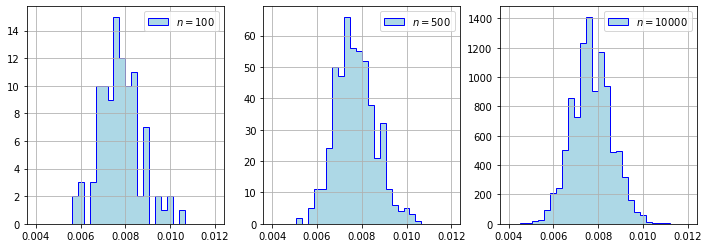
\includegraphics[width=1\textwidth]{figures/lesson4_25_0.png}
	\caption{Evolution of the distribution of $\mu_n$ with the increase of
	the number of MC experiments (100, 500, 10000).}
\label{fig:repeated_MC}
\end{figure}

Looking at Fig.~\ref{fig:repeated_MC} it is clear how increasing the number of
experiments the distribution of the results becomes more and more Gaussian-like.
From the central limit theorem hence: 

\begin{equation}
\mu_n - \mu \approx \mathcal{N}(0, \sigma^2/n)
\end{equation}

\begin{figure}[tb]
	\centering
	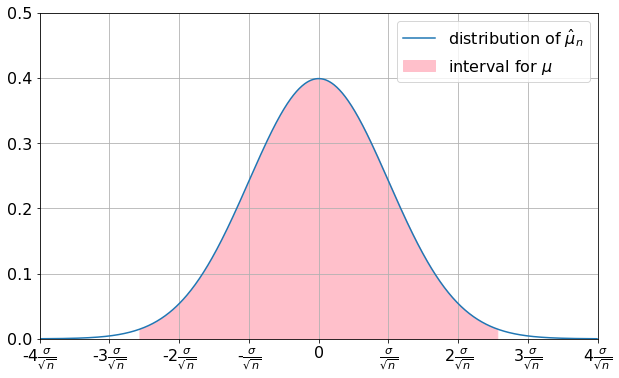
\includegraphics[width=0.7\textwidth]{figures/confidence_interval.png}
	\caption{Confidence interval for a MC experiment.}
	\label{fig:confidence_interval}
\end{figure}

Considering one single Monte Carlo experiment we can define an
interval so that there is a certain probability to find \(\mu\) in
there. Referring to Fig.~\ref{fig:confidence_interval} we can write:

\begin{equation}
P\left(\mu_n - \cfrac{1.96\sigma}{\sqrt{n}}\le \mu \le \mu_n + \cfrac{1.96\sigma}{\sqrt{n}}\right) = 0.95
\end{equation}
probability which correspond to the shaded area.

This interval is called \textbf{95\% confidence interval} because
it covers 95\% of the total area under the Gaussian. It can be
interpreted like the following: if you repeat many times the simulation, 
the fraction of calculated confidence intervals that contains the true
parameter \(\mu\) would tend toward 95\%.

The most commonly used intervals are 99\% and 95\% confidence level and are
respectively defined as \(\pm \cfrac{2.57\sigma}{\sqrt{n}}\) and
\(\pm \cfrac{1.96\sigma}{\sqrt{n}}\).

To construct an interval with a custom confidence level $\alpha$, we have to find a number $A$ such that
\begin{equation}
\Phi(A) = 1 - \frac{1-\alpha}{2}\quad\implies\quad A = \Phi^{-1}\left(\cfrac{1+\alpha}{2}\right)
\label{for:A}
\end{equation}
then the $\alpha$-confidence interval guarantees
\begin{equation}
P(\mu - A\sigma \le X \le \mu+ A\sigma) = \alpha 
\end{equation}

Below an example of how to compute a confidence level in \texttt{python} given a set of fake simulations. To note that the inverse of the Gaussian CDF ($\Phi^{-1}$), used in Equation~\ref{for:A}, is computed with the method \texttt{norm.ppf()} (more details on CDF in Chapter~\ref{quantile-function}).

\begin{tcolorbox}[breakable, size=fbox, boxrule=1pt, pad at break*=1mm,colback=cellbackground, colframe=cellborder]
\begin{Verbatim}[commandchars=\\\{\}]
\PY{k+kn}{import} \PY{n+nn}{numpy} \PY{k}{as} \PY{n+nn}{np}
\PY{k+kn}{from} \PY{n+nn}{scipy}\PY{n+nn}{.}\PY{n+nn}{stats} \PY{k}{import} \PY{n}{norm}
	
\PY{n}{samples} \PY{o}{=} \PY{p}{[}\PY{l+m+mf}{1.}\PY{p}{,}\PY{l+m+mf}{2.}\PY{p}{,}\PY{l+m+mf}{3.}\PY{p}{,}\PY{l+m+mf}{4.}\PY{p}{,}\PY{l+m+mf}{4.}\PY{p}{,}\PY{l+m+mf}{4.}\PY{p}{,}\PY{l+m+mf}{5.}\PY{p}{,}\PY{l+m+mf}{5.}\PY{p}{,}\PY{l+m+mf}{5.}\PY{p}{,}\PY{l+m+mf}{5.}\PY{p}{,}\PY{l+m+mf}{4.}\PY{p}{,}\PY{l+m+mf}{4.}\PY{p}{,}\PY{l+m+mf}{4.}\PY{p}{,}\PY{l+m+mf}{6.}\PY{p}{,}\PY{l+m+mf}{7.}\PY{p}{,}\PY{l+m+mf}{8.}\PY{p}{]}
\PY{n}{alpha} \PY{o}{=} \PY{l+m+mf}{0.95}
	
\PY{n}{X} \PY{o}{=} \PY{n}{np}\PY{o}{.}\PY{n}{array}\PY{p}{(}\PY{n}{samples}\PY{p}{)}
\PY{n}{A} \PY{o}{=} \PY{n}{norm}\PY{o}{.}\PY{n}{ppf}\PY{p}{(}\PY{p}{(}\PY{l+m+mi}{1} \PY{o}{+} \PY{n}{alpha}\PY{p}{)}\PY{o}{/}\PY{l+m+mi}{2}\PY{p}{)}
\PY{n}{m}\PY{p}{,} \PY{n}{se} \PY{o}{=} \PY{n}{np}\PY{o}{.}\PY{n}{mean}\PY{p}{(}\PY{n}{X}\PY{p}{)}\PY{p}{,} \PY{n}{np}\PY{o}{.}\PY{n}{std}\PY{p}{(}\PY{n}{X}\PY{p}{)}
\PY{n}{h} \PY{o}{=} \PY{n}{A}\PY{o}{*}\PY{n}{se}\PY{o}{/}\PY{n}{np}\PY{o}{.}\PY{n}{sqrt}\PY{p}{(}\PY{n+nb}{len}\PY{p}{(}\PY{n}{samples}\PY{p}{)}\PY{p}{)}
\PY{n+nb}{print} \PY{p}{(}\PY{l+s+s2}{\PYZdq{}}\PY{l+s+si}{\PYZob{}:.0f\PYZcb{}}\PY{l+s+si}{\PYZpc{} c}\PY{l+s+s2}{onfidence interval: }\PY{l+s+si}{\PYZob{}\PYZcb{}}\PY{l+s+s2}{ +\PYZhy{} }\PY{l+s+si}{\PYZob{}\PYZcb{}}\PY{l+s+s2}{\PYZdq{}}\PY{o}{.}\PY{n}{format}\PY{p}{(}\PY{n}{alpha}\PY{o}{*}\PY{l+m+mi}{100}\PY{p}{,} \PY{n}{m}\PY{p}{,} \PY{n}{h}\PY{p}{)}\PY{p}{)}
	
95\% confidence interval: 4.4375 +- 0.8119808363806419
\end{Verbatim}
\end{tcolorbox}

The confidence interval can be used to assess the accuracy of the Monte
Carlo simulation. The root mean squared error on our best estimate of
\(\mu\) is:

\[ \mathrm{RMSE}(\mu_n) = \sqrt{\mathbb{E}((\mu_n - \mu )^2)} = \sqrt{\cfrac{\sigma^2}{n}}=\cfrac{\sigma}{\sqrt{n}} \]
where \(\sigma^2 = \mathrm{Var}(Y)\).

While it is obvious that the estimate should get worse with increased variance and better with increased sample size, this equation  gives us the exact rate of exchange. Indeed the RMSE tells us that to get one more decimal digit of accuracy (i.e. an RMSE one tenth as large) requires a 100-fold increase in computation. To get three more digits of accuracy requires one million times as much computation. From that it is clear that Monte Carlo computation is poorly suited for problems that must be answered with high precision.


\chapter{Stochastic Processes}

In financial engineering simulation tools have been increasingly gaining 
importance due to both the continuous enhancement of computational efficiency 
and the development of very complex financial, especially derivative
instruments.

A model of the dynamics of asset prices must reflect the random nature
of price movements. Stock prices are usually assumed to follow a 
\emph{Markov process}. Markov processes can be characterized as a
particular type of stochastic processes without any history. Past values
and the way the present has emerged from the past are therefore
irrelevant. 

A particular type of a Markov stochastic
process and presumably the simplest process is the so called Wiener
process or elementary Brownian motion, $\Delta W = z\sqrt{\Delta t}$, where z is 
assumed to be iid1 and $z ∼ \phi (0, 1)$. The mean of $\Delta W$ is zero and its variance is 
$\Delta t$, which means the standard deviation grows with the square root of time.
It follows that $W(t) ∼ \phi (0, t)$. Since it is common to
proceed from small changes to the limit, $\Delta W$ goes to $dW$ as $\Delta t \rightarrow 0$.

If we allow for a drift and variance rate, the process $X(t)$ is called an
arithmetic Brownian motion with drift $\mu$ and diffusion coefficient $\sigma^2$ if
independent and identically distributed 

\begin{equation}
	\cfrac{X(t) − \mu t}{\sigma} 
\end{equation}
follows an elementary Brownian motion. Thus $X(t) ∼ \phi(\mu t, \sigma^t)$ 
and $X$ solves the stochastic differential equation (SDE) 

dX(t)
= μdt + σdW(t). (1.16) Note that the parameters μ and σ are
deterministic and independent of both the time t and the variable X. If
we allow them to be time-varying and dependent on the level of X, the
result will be an Itˆo process {[}56, p.269{]} dX(t) =
μ(X,t)dt+σ(X,t)dW(t). Because Brownian motion increments are
independently normally distributed, simulating W(t) or X(t) is
straightforward. Since an arithmetic Brownian motion can also take
negative values, this type of process is apparently unsuitable for
simulating asset prices. These are rather assumed to follow a geometric
Brownian motion (GBM). A stochastic process S(t) is regarded as a GBM,
abbreviated S(t) ∼ GBM(μ,σ2), if lnS(t) is a Brownian motion with
initial value lnS(0) {[}46, p.93{]}. In this case we would write a GBM
as S(t) = S(0) + or in shorthand and divided by S(t), 􏰑t 􏰑t μSudu + 00
σSudWu

dS (t) S(t) =μdt+σdW(t). A GBM is one of the most fundamental models to
describe the evolution of the value of financial assets. The SDE defined
by Equation (1.17) is well-defined. The first integral on the right-hand
side is a regular Riemann integral and the second integral is a
stochastic, or also called Itˆo integral. Note that the left-hand side
of Equation (1.18) represents the proportional change in the asset price
in the interval (t, t + dt) and additionally shows that dS/S ∼ φ(μdt,
σ2dt) {[}46, p.93{]}. Applying Itˆo's lemma (see Section 1.2.2) one can
find the following solution 1 S(t)=S(0)exp((μ− 2σ2)t+σW(t)) (1.19) for
the SDEs (1.17) and (1.18), respectively. Equation (1.19) allows us now
to simulate an arbitrary number of possible asset price paths by Monte
Carlo. Particularly, a random path for an asset price can be simulated
by sampling repeatedly for z from φ(0,1) and substituting in Equation
(1.19). It follows that the logarithm of the asset price is thus
normally distributed, and the price itself has a lognormal distribution
{[}56, p.275{]}. The source of this normality lies in the Wiener
process, which is a reasonable assumption due to the central limit
theorem. Figure 2 shows possible asset price paths that are assumed to
follow a geometric Brownian motion with the parameters S(0) = 100, μ =
0.05, σ = 0.4, t = 1 and dt = 1/365. The simulated asset prices in one
year are S(t)1 = 134.72, S(t)2 = 72.12 and S(t)3 = 62.20.

1.2.2 Pricing vanilla European options by Monte Carlo Having generated
the sample paths of asset prices under the assumption of a certain
diffusion process, only small steps bring us to the pricing of
derivative instruments using Monte Carlo. The doubtless most important
one was firstly taken by Kiyoshi Itˆo in 1951 when he published Itˆo's
lemma 􏰅∂G ∂G 1∂2G 􏰆 ∂G dG = μ + + σ2 dt + σdW (1.20) ∂x ∂t 2∂x2 ∂x in
the article On Stochastic Differential Equations {[}58{]}, where G is a
continuous and differentiable function of the variable x. He basically
showed by a simple Taylor series expansion that, firstly, the term
involving ∆x2 in Equation (1.20) includes a component of order ∆t and
therefore must not be ignored as ∆t → 0. Secondly, the variance of z2∆t
is of order ∆t2 and therefore ∆x2 becomes nonstochastic and equal to
σ2dt as ∆t → 0 {[}56, p.279-280{]}. A price of derivatives is eventually
a function of the underlying asset's price and time. Ap- plying Itˆo's
lemma, we can calculate the stochastic process followed by a function
whose inputs come from the stochastic process followed by the underlying
itself {[}56, p.273ff{]}. Thus with Itˆo's lemma in our toolbox we are
able to understand the dynamics of derivatives. A key point to keep in
mind is that the Wiener process underlying the stochastic process for
the asset price is exactly the same as the Wiener process underlying the
stochastic process for the derivative. Therefore, both are subject to
the same source of uncertainty, which is of prime importance not only
for the application of Monte Carlo but also for the entire option
pricing theory. Let us now consider the application of Monte Carlo to a
vanilla European call option. This may seem a little pointless, as there
is with Black-Scholes {[}9{]} an analytical method that delivers the
true option price much easier. Nevertheless, it builds a good and easy
introduction to identify the exact Monte Carlo procedure. The payoff of
a call option with strike K and duration T is (S(T)−K)+
=max\{0,S(T)−K\}. (1.21) 9 Asset price 1 Fundamentals By multiplying
this payoff by a discount factor e−rT we get the present value of the
payoff. This is commonly done with a continuously compounded risk-free
interest rate, denoted as r. The expected present value and thus the
call option price C is defined by {[}46, p.4{]} C = e−rT E{[}(S(T) −
K)+{]}. However, without the knowledge of any distributional
characteristics of the random variable S(T), this expectation is totally
meaningless. It is impossible to price an option without any information
about its distribution of the underlying price or its return. Therefore,
we necessarily need to specify the particular distribution of the final
asset price S(T). In the previous section a model for the dynamics of
stock prices, namely the geometric Brownian motion, was introduced. This
model provides us with the lognormal distribution of S(T), the required
information for a successful option pricing via expected values. Since
we are in a risk-neutral environment2, the drift parameter μ in Equation
(1.19) may be replaced by the risk-free rate r. Hence it is
straightforward to find the asymptotically correct value for the
European call option by Monte Carlo simulation. In a first step,
simulate one path for the asset price as it is done in Figure 2 and
calculate, according to (1.21), the corresponding payoff. Secondly,
repeat this first step numerous times which provides you with several
payoffs. Third and last step, compute the mean payoff and multiply it
with the risk-free discount factor. For any n ≥ 1, the Monte Carlo
estimator Cˆ is unbiased and strongly consistent, in the sense that its
expectation n E{[}Cˆ {]} = C ≡ e−rT E{[}(S(T) − K)+{]}, n ˆ meaning that
lim Cn = C {[}46, p.4f{]}. n→∞ The fact that this Monte Carlo estimator
is indeed consistent is illustrated in Figure 3. The ˆ figure shows the
development of the relative pricing error, computed as (Cn − C)/C, with
a steadily growing sample n.~Note that the pricing error is gradually
decreasing and eventually converting to 0 as n goes to infinity. This is
a first proof that Monte Carlo provides correct results in the limit and
is basically the prerequisite for its increasing importance in valuing
derivatives.









\section{Derivation of log-normal Stochastic Differential
	Equation}\label{derivation-of-log-normal-stochastic-differential-equation}


In this Section we will see how to implement the simulation of a stock price which deviates from a steady state as a result of random fluctuations given by the trades. 

Considering a stock with a price \(S_t\) and its expected rate of return \(\mu\); the relative change in its price during a period \(dt\) can be decomposed in two parts

\begin{itemize}
\tightlist
\item
  a deterministic part: that is the expected return from the stock held
  during the time period \(dt\) and which can be expressed as \(\mu S_tdt\)
\item
  a stochastic part: which reflects the random changes of the market
  (e.g. as a response to external effects such as unexpected news). A
  reasonable assumption is to take this contribution proportional to the
  stock so \(\sigma S_t dB_t\), where \(dB_t\) is a so called random walk process equal to \(\epsilon\sqrt{t}=\mathcal{N}(0,1)\sqrt{t}\).
\end{itemize}
Putting the two contributions together the resulting differential equation is:

\begin{equation}
  dS_t = \mu S_tdt + \sigma S_tdB_t
  \label{eq:differential}
\end{equation}
or dividing by $S_t$
\begin{equation}
\frac{dS_t}{S_t} = d\textrm{log}(S_t) = \mu dt + \sigma dB_t
\end{equation}

The solution of this equation can be derived by applying the
It\(\hat{o}\)'s formula which states that for any given function
\(G(S, t)\) where \(S\) satisfies the following stochastic differential
equation \(dS=a\cdot dt +b\cdot dB_t\) it holds:

\begin{equation}
dG=\big(a\frac{\partial G}{\partial S} + \frac{\partial G}{\partial t} + \frac{1}{2}b^2\frac{\partial^2 G}{\partial S^2} \big)dt + b \frac{\partial G}{\partial S}dB
\label{eq:itos_lemma}
\end{equation}

Now if we set \(G = \textrm{log}(S_t)\) we can compute the derivatives:

\begin{equation}
\begin{gathered}
\frac{\partial G}{\partial S} = \frac{1}{S_t}\\
\frac{\partial G}{\partial t} = 0\\
\frac{\partial^2 G}{\partial S^2} = -\frac{1}{S_t^{2}}
\end{gathered}
\end{equation}

Substituting back into Eq.~\ref{eq:itos_lemma} and taking the values of $a$ and $b$ from Eq.~\ref{eq:differential} we get:

\begin{equation}
\begin{gathered}
d(\textrm{log} S_t) = \big(\mu S_t \cfrac{1}{S_t} + \cfrac{1}{2}\sigma^2 S_t^2 (-\cfrac{1}{S_t^2})\big)dt + \sigma\epsilon\sqrt{dt}\\
d(\textrm{log} S_t) = \textrm{log} (S_t) - \textrm{log} (S_{t-1}) = \textrm{log} \cfrac{S_t}{S_{t-1}} = \big(\mu - \cfrac{1}{2}\sigma^2\big)dt + \sigma\epsilon\sqrt{dt}\\
S_t = S_{t-1}e^{\big(\mu - \cfrac{1}{2}\sigma^2\big)dt + \sigma\epsilon\sqrt{dt}}
\end{gathered}
\end{equation}

As can be seen from the following equation:

\begin{equation}
d(\textrm{log} S_t) = \big(\mu - \cfrac{1}{2}\sigma^2\big)dt + \sigma\epsilon\sqrt{dt}
\end{equation}
the change in \(\textrm{log} S_t\) has a constant \emph{drift} with respect to time \(\mu - \frac{1}{2}\sigma^2\) and a constant variance rate \(\sigma^2\)
(remember that \(\epsilon\) is a normally distributed random variable
\(\mathcal{N}(0,1)\)). So you have a constant plus a Gaussian
distributed variable, therefore \(\textrm{log} S_t\) at some time \(T\)
is normally distributed with:

\begin{equation}
\textrm{log}S_t - \textrm{log}S_0 \approx\mathcal{N}\big[\big(\mu-\frac{\sigma^2}{2}\big)T, \sigma^2 T\big]
\end{equation}

This equation shows that \(\textrm{log}S_t\) is normally distributed,
and \textbf{such a variable whose logarithm is normally distributed is said
to be log-normal}. 

The model we have just developed implies that
the stock price at time T, given today's price, is log-normally
distributed. One of the nicer properties of a log-normal distribution is to be positive defined and that's why log-normality is an important characteristic for stole prices: we need to \emph{ensure} that will never be negative. 

Actually this result was expected, in fact looking at the initial \(dS\) equation (Eq.~\ref{eq:differential}) we had:

\begin{equation}
dS_t = \mu S_tdt + \sigma S_tdB_t
\end{equation}
which shows that the closer \(S_t\) is to 0, the smaller is its variation \(dS\), so it will never go negative.

\subsection{Simulation of a Stock Price}

Now that we are able to approximate the course of a stock price, let's implement a simulation.

\begin{tcolorbox}[breakable, size=fbox, boxrule=1pt, pad at break*=1mm,colback=cellbackground, colframe=cellborder]
\begin{Verbatim}[commandchars=\\\{\}]
\PY{k+kn}{from} \PY{n+nn}{numpy}\PY{n+nn}{.}\PY{n+nn}{random} \PY{k}{import} \PY{n}{normal}\PY{p}{,} \PY{n}{seed} 
\PY{k+kn}{from} \PY{n+nn}{matplotlib} \PY{k}{import} \PY{n}{pyplot} \PY{k}{as} \PY{n}{plt} 
\PY{k+kn}{import} \PY{n+nn}{math}
		
\PY{c+c1}{\PYZsh{}initial price}
\PY{n}{S} \PY{o}{=} \PY{l+m+mi}{100}
\PY{n}{mu} \PY{o}{=} \PY{o}{\PYZhy{}}\PY{l+m+mf}{0.01} 
\PY{n}{sigma} \PY{o}{=} \PY{l+m+mf}{0.05} 
\PY{n}{T}\PY{o}{=}\PY{l+m+mi}{1}
\PY{n}{seed}\PY{p}{(}\PY{l+m+mi}{1}\PY{p}{)} 
\PY{n}{historical\PYZus{}series} \PY{o}{=} \PY{p}{[}\PY{n}{S0}\PY{p}{]}
\PY{c+c1}{\PYZsh{} 30 days simulation}
\PY{k}{for} \PY{n}{i} \PY{o+ow}{in} \PY{n+nb}{range}\PY{p}{(}\PY{l+m+mi}{30}\PY{p}{)}\PY{p}{:}
    \PY{n}{S} \PY{o}{=} \PY{n}{S} \PY{o}{*} \PY{n}{math}\PY{o}{.}\PY{n}{exp}\PY{p}{(}\PY{p}{(}\PY{n}{mu} \PY{o}{\PYZhy{}} \PY{l+m+mf}{0.5} \PY{o}{*} \PY{n}{sigma} \PY{o}{*} \PY{n}{sigma}\PY{p}{)} \PY{o}{*} \PY{n}{T} \PY{o}{+}
    \PY{n}{sigma} \PY{o}{*} \PY{n}{math}\PY{o}{.}\PY{n}{sqrt}\PY{p}{(}\PY{n}{T}\PY{p}{)} \PY{o}{*} \PY{n}{normal}\PY{p}{(}\PY{p}{)}\PY{p}{)}
    \PY{n}{historical\PYZus{}series}\PY{o}{.}\PY{n}{append}\PY{p}{(}\PY{n}{S}\PY{p}{)}
\end{Verbatim}
\end{tcolorbox}
The result of the simulation is shown in Fig.~\ref{fig:stock_price_sim}.

\begin{figure}[b]
	\centering
	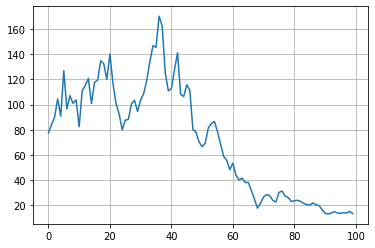
\includegraphics[width=0.7\textwidth]{figures/lesson4_29_0.png}
	\caption{Simulation with Monte Carlo method of a stock price, using the log-normal evolution.}
	\label{fig:stock_price_sim}
\end{figure}


